\documentclass[a4paper,11pt]{article}
\usepackage[utf8]{inputenc}
\usepackage[english]{babel}
\usepackage{geometry}
\usepackage{enumitem}
\usepackage{hyperref}
\usepackage{xcolor}
\usepackage{tcolorbox}
\usepackage{amsmath} 
\usepackage{graphicx}
\usepackage{titling}
\usepackage{tikz}
\usetikzlibrary{calc}
\usepackage{float}
\geometry{margin=2.5cm}

% ===== Data matkul (silakan sesuaikan) =====
\newcommand{\KodeMK}{CSCE604029}
\newcommand{\NamaMK}{Computer Graphics}
\newcommand{\SemesterTahun}{Semester Gasal 2025/2026}
\newcommand{\Institusi}{Fakultas Ilmu Komputer, Universitas Indonesia}

% ===== Gambar header tunggal =====
\newcommand{\HeaderImage}{images/header-fasilkom-ui.png}

% ===== Judul & deadline =====
\title{\textbf{Assignment 1: Raterization Pipeline}}
\author{} % tidak dipakai
\date{Deadline: 2 October 2025 pukul 23.59 WIB}

% ===== Style judul =====
\definecolor{deadlineRed}{RGB}{200,0,0}
\pretitle{\vspace{-1.0cm}}
\renewcommand{\maketitle}{%
  \begin{center}
    % gambar header dibuat lebih kecil
    \includegraphics[width=0.45\linewidth]{\HeaderImage}
  \end{center}
  \vspace{2mm}
  \begin{center}
    {\Large\bfseries \KodeMK\ $\bullet$ \NamaMK}\\
    {\large\bfseries \SemesterTahun}\\
    {\large\bfseries \Institusi}
  \end{center}
  \vspace{3mm}
  \begin{center}
    {\Large\bfseries \thetitle}\\[2mm]
    {\normalsize\textcolor{deadlineRed}{\textbf{\thedate}}}
  \end{center}
  \vspace{4mm}\hrule\vspace{6mm}
}

\begin{document}
\maketitle

\begin{tcolorbox}[
    title=Alignment with CPMK,
    colback=blue!5!white,
    colframe=blue!50!black,
    fonttitle=\bfseries,
]
\begin{itemize}
    \item Menguasai konsep-konsep dasar grafika komputer secara teoritis seperti model kamera, properti warna dan cahaya, rendering, iluminasi, dan geometri.
    \item Dapat mendesain solusi grafika komputer untuk pembentukan citra digital menggunakan teknik pemodelan dasar, terutama menggunakan metode berbasis rasterization dan ray tracing.
\end{itemize}
\end{tcolorbox}

% Material Explanation Section for SVG Rasterizer Assignment
% This content should be inserted into the main.tex file

\section{Introduction}

This assignment focuses on implementing a \textbf{2D SVG software rasterizer}, which is a fundamental computer graphics system that converts vector graphics into pixel images. Unlike hardware-accelerated rendering (GPU-based), software rasterization is performed entirely on the CPU, giving you direct control over every pixel and a deep understanding of the rendering pipeline.

\begin{figure}[H]
    \centering
    \includegraphics[width=0.25\linewidth]{images/rasterization.png}
    \caption{Rasterized Vector Triangle}
    \label{fig:placeholder}
\end{figure}

\subsection{What is Rasterization?}

Rasterization is the process of converting geometric primitives (lines, triangles, curves) defined in continuous coordinate spaces into discrete pixels on a screen or image buffer. This process involves several key challenges:

\subsubsection{Coordinate Transformation}

In 2D computer graphics several coordinate systems are used in sequence. Object (local) space is where a shape is defined (for example, a unit circle at the origin). World (canvas) space places all shapes together by translation, rotation, and scaling. Normalized Device Coordinates (NDC) are a resolution-independent square \([-1,1]\times[-1,1]\) obtained after a viewing/normalization step so geometry no longer depends on pixel dimensions. Screen space consists of integer pixel coordinates \([0,W)\times[0,H)\) on the final image.

All stages are affine transforms in homogeneous 2D, represented by \(3\times3\) matrices. If \(\mathbf M\) maps object\(\to\)world, \(\mathbf V\) maps world\(\to\)NDC, and \(\mathbf S\) maps NDC\(\to\)screen, then for a point \(\mathbf p=(x,y,1)^{\mathsf T}\):
\[
\mathbf p_{\text{screen}}=\mathbf S\,\mathbf V\,\mathbf M\,\mathbf p.
\]
A convenient 2D normalization is to translate the window center \((x,y)\) to the origin and scale by \(1/\text{span}\) so the square \([x-\text{span},x+\text{span}]\times[y-\text{span},y+\text{span}]\) maps to \([-1,1]^2\):
\[
\mathbf V_{\!2D} =
\begin{bmatrix}
\frac{1}{\text{span}} & 0 & -\frac{x}{\text{span}}\\[4pt]
0 & \frac{1}{\text{span}} & -\frac{y}{\text{span}}\\[4pt]
0 & 0 & 1
\end{bmatrix}.
\]
The viewport matrix \(\mathbf S\) then maps NDC \((u,v)\in[-1,1]^2\) to pixels:
\[
x_{\text{pix}}=\tfrac{W}{2}(u+1),\qquad y_{\text{pix}}=\tfrac{H}{2}(v+1).
\]
Matrix multiplication order and the chosen row/column convention must be consistent to avoid unintended flips or offsets.

Textbook/OpenGL diagrams often show \emph{local} \(\to\) \emph{world} \(\to\) \emph{view} \(\to\) \emph{clip} \(\to\) \emph{screen}. In 3D, a view matrix re-expresses coordinates in camera space and a projection matrix sends them to clip space; NDC are obtained after the perspective divide. In our 2D orthographic setting there is no perspective, so clip \(=\) NDC and the “camera” reduces to a world-window normalization. Consequently we fold view\(+\)projection into \(\mathbf V_{\!2D}\), yielding the shorter chain object \(\to\) world \(\to\) NDC \(\to\) screen used here.

\begin{figure}[H]
  \centering
  \includegraphics[width=0.72\linewidth]{images/coordinate-transform.png}
  \caption{Common 3D pipeline (local $\rightarrow$ world $\rightarrow$ view $\rightarrow$ clip $\rightarrow$ screen). 
  In 2D orthographic rendering we fold view+projection into a single normalization \(\mathbf V_{\!2D}\), so clip \(=\) NDC and the chain simplifies to object $\rightarrow$ world $\rightarrow$ NDC $\rightarrow$ screen.}
  \label{fig:coord-transform}
\end{figure}

\vspace{0.75em}
\subsubsection{Primitive Decomposition}

Rendering is most robust when complex 2D shapes are reduced to triangles. Any convex quadrilateral becomes two triangles; a simple (non self-intersecting) polygon can be tessellated with ear clipping. Triangles are always convex and determined by three points, so inside tests are straightforward and attribute interpolation (for colors or texture coordinates) is well behaved. Once shapes are represented as a triangle list, a single triangle routine can handle all filled geometry.

\begin{figure}[H]
    \centering
    \includegraphics[width=0.25\linewidth]{images/ear-clipping.png}
    \caption{Ear clipping triangulation}
    \label{fig:placeholder}
\end{figure}

\vspace{0.75em}
\subsubsection{Pixel Coverage}

Determining whether a discrete sample lies inside a continuous triangle can be done efficiently with edge functions. For vertices \(v_0, v_1, v_2\) and any point \(p\),
\[
E_{ab}(p)=(p-a)\times(b-a)=(p_x-a_x)(b_y-a_y)-(p_y-a_y)(b_x-a_x).
\]
The signed twice-area is \(A=E_{01}(v_2)\). For each sample center \(p=(x+0.5,y+0.5)\) inside a conservative integer bounding box, evaluate \(E_{01}(p),E_{12}(p),E_{20}(p)\); if they share the sign of \(A\), the sample is inside. Barycentric coordinates follow directly,
\[
(\alpha,\beta,\gamma)=\tfrac{1}{A}\big(E_{12}(p),E_{20}(p),E_{01}(p)\big),\qquad \alpha+\beta+\gamma=1,
\]
and are useful for interpolating per-vertex attributes. Degenerate cases with \(|A|\approx 0\) are treated as empty.

\begin{figure}[h]
\centering
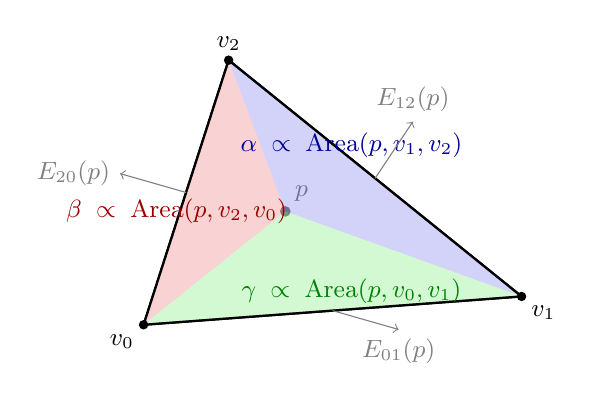
\begin{tikzpicture}[scale=1.2, every node/.style={font=\small}]
  % Vertices of the main triangle
  \coordinate (v0) at (0,0);
  \coordinate (v1) at (4,0.3);
  \coordinate (v2) at (0.9,2.8);

  % Outline and light fill of the main triangle
  \fill[black!5] (v0)--(v1)--(v2)--cycle;
  \draw[thick] (v0)--(v1)--(v2)--cycle;

  % Interior point p
  \coordinate (p) at (1.5,1.2);
  \filldraw[black] (p) circle (0.05) node[above right] {$p$};

  % Sub-triangles showing areas proportional to barycentric weights
  % alpha corresponds to area opposite v0: Area(p, v1, v2)
  \fill[blue!25, opacity=0.6] (p)--(v1)--(v2)--cycle;
  % beta corresponds to area opposite v1: Area(p, v2, v0)
  \fill[red!25, opacity=0.6]  (p)--(v2)--(v0)--cycle;
  % gamma corresponds to area opposite v2: Area(p, v0, v1)
  \fill[green!25, opacity=0.6] (p)--(v0)--(v1)--cycle;

  % Re-draw main triangle border on top
  \draw[thick] (v0)--(v1)--(v2)--cycle;

  % Vertex markers and labels
  \fill (v0) circle (0.05) node[below left] {$v_0$};
  \fill (v1) circle (0.05) node[below right] {$v_1$};
  \fill (v2) circle (0.05) node[above] {$v_2$};

  % Annotate which area maps to which weight
  \node[blue!60!black]  at (2.2,1.9) {$\alpha \;\propto\; \mathrm{Area}(p,v_1,v_2)$};
  \node[red!60!black]   at (0.35,1.2) {$\beta \;\propto\; \mathrm{Area}(p,v_2,v_0)$};
  \node[green!50!black] at (2.2,0.35) {$\gamma \;\propto\; \mathrm{Area}(p,v_0,v_1)$};

  % Optional: indicate edge-function names near edges (light gray)
  \draw[->, gray] ($(v1)!0.5!(v2)$) -- ++(0.4,0.6) node[gray, above] {$E_{12}(p)$};
  \draw[->, gray] ($(v2)!0.5!(v0)$) -- ++(-0.7,0.2) node[gray, left] {$E_{20}(p)$};
  \draw[->, gray] ($(v0)!0.5!(v1)$) -- ++(0.7,-0.2) node[gray, below] {$E_{01}(p)$};
\end{tikzpicture}

\vspace{2mm}
\footnotesize
$\displaystyle
\alpha=\frac{\mathrm{Area}(p,v_1,v_2)}{\mathrm{Area}(v_0,v_1,v_2)},\quad
\beta=\frac{\mathrm{Area}(p,v_2,v_0)}{\mathrm{Area}(v_0,v_1,v_2)},\quad
\gamma=\frac{\mathrm{Area}(p,v_0,v_1)}{\mathrm{Area}(v_0,v_1,v_2)},\quad
\alpha+\beta+\gamma=1.
$
\end{figure}

\vspace{0.75em}
\subsubsection{Anti-aliasing}


Aliasing occurs when continuous geometry is sampled too coarsely, producing stair-steps (jaggies) and moiré. Supersampling anti-aliasing (SSAA) addresses this by subdividing each pixel into an \(N\times N\) grid of sub-pixel samples. Rasterization is evaluated at these sample positions; a resolve step then averages the \(N^2\) samples back into one pixel using a box reconstruction filter:
\[
C_{\text{pixel}}=\frac{1}{N^2}\sum_{i=1}^{N^2} C_{\text{sample},i}.
\]
Accurate results depend on sampling at well-defined centers, carefully converting between pixel indices and sub-sample indices (\(x_s=x\cdot N+s_x\)), and clamping indices to valid ranges to avoid out-of-bounds writes. SSAA trades additional work and memory for smoother edges and reduced artifacts.

\begin{figure}[H]
    \centering
    \includegraphics[width=0.5\linewidth]{images/aliasing.png}
    \caption{Comparison between Aliasing and using Anti-Aliasing}
    \label{fig:placeholder}
\end{figure}

\vspace{0.75em}
\subsubsection{Color Blending}

Transparency is modeled by storing an opacity value \(\alpha\in[0,1]\) alongside color \(C\). With straight (non-premultiplied) alpha, the standard source-over composition for foreground \((C_f,\alpha_f)\) over background \((C_b,\alpha_b)\) is
\[
C_{\text{out}}=\alpha_f\,C_f+(1-\alpha_f)\,C_b,\qquad
\alpha_{\text{out}}=\alpha_f+(1-\alpha_f)\,\alpha_b.
\]
This operation is applied per sample, and draw order determines which layers appear on top. Blending should be performed in a linear color space; any gamma correction is applied later when converting final resolved pixels for display.


\subsection{Core Rasterization Concepts}

Rasterization converts a scene described by continuous geometry and styles into a finite grid of colored pixels. The core ideas span (i) how coordinates move through spaces via linear/affine transforms, (ii) how we decide which discrete samples belong to a primitive (coverage), (iii) how we reduce aliasing by sampling more densely than one sample per pixel, (iv) how colors combine when layers overlap (alpha compositing), and (v) how images are sampled and filtered when used as textures. This subsection develops the first piece—coordinate systems and transformations—because every later stage consumes geometry that has been coherently mapped to a common image space.

\subsubsection{Coordinate Systems and Transformations}

A coordinate system specifies an origin and axes against which points are measured. In 2D graphics we routinely pass through several systems so that each operation happens where it is most natural. Shapes are authored in object (local) space, placed into a scene in world (canvas) space, normalized to a resolution-independent square called Normalized Device Coordinates (NDC), and finally mapped to integer screen-space pixels. For 2D orthographic rendering there is no perspective foreshortening, so clip space coincides with NDC.

All of these steps are expressed as affine transforms in homogeneous coordinates using \(3\times 3\) matrices. Writing a 2D point as \(\mathbf p=(x,y,1)^{\mathsf T}\),
\[
\mathbf p_{\text{screen}} = \mathbf S\,\mathbf V\,\mathbf M\,\mathbf p_{\text{object}},
\]
where \(\mathbf M\) positions the object in world space, \(\mathbf V\) normalizes a chosen world window into NDC, and \(\mathbf S\) maps NDC to pixel coordinates. With column vectors the order matters: the rightmost transform applies first. Being consistent about this convention avoids mirrored or shifted results.

Translation, rotation, and anisotropic scaling are the building blocks:
\[
\mathbf T(t_x,t_y)=
\begin{bmatrix}
1&0&t_x\\[2pt]0&1&t_y\\[2pt]0&0&1
\end{bmatrix},\qquad
\mathbf R(\theta)=
\begin{bmatrix}
\cos\theta&-\sin\theta&0\\[2pt]\sin\theta&\cos\theta&0\\[2pt]0&0&1
\end{bmatrix},\qquad
\mathbf S(s_x,s_y)=
\begin{bmatrix}
s_x&0&0\\[2pt]0&s_y&0\\[2pt]0&0&1
\end{bmatrix}.
\]
Any affine map is a product of these (and optionally a shear). Composition is associative but not commutative, so \(\mathbf R\,\mathbf T \neq \mathbf T\,\mathbf R\) in general. The model matrix \(\mathbf M\) places an object authored near \((0,0)\) into the scene, e.g., \(\mathbf M=\mathbf T\,\mathbf R\,\mathbf S\). 

World coordinates are normalized to NDC by mapping a world window
\([x-\mathrm{span},\,x+\mathrm{span}]\times[y-\mathrm{span},\,y+\mathrm{span}]\)
to the fixed square \([-1,1]\times[-1,1]\). One convenient matrix is
\[
\mathbf V =
\begin{bmatrix}
\frac{1}{\mathrm{span}} & 0 & -\frac{x}{\mathrm{span}}\\[4pt]
0 & \frac{1}{\mathrm{span}} & -\frac{y}{\mathrm{span}}\\[4pt]
0 & 0 & 1
\end{bmatrix},
\]
which first translates the window center \((x,y)\) to the origin and then scales by \(1/\mathrm{span}\) equally in \(x\) and \(y\). If the image’s aspect ratio is not square, either choose different spans per axis, or apply an additional scale to preserve circles as circles in NDC.

The viewport then converts \((u,v)\in[-1,1]^2\) to integer pixel coordinates for an image of width \(W\) and height \(H\):
\[
x_{\text{pix}}=\frac{W}{2}(u+1),\qquad y_{\text{pix}}=\frac{H}{2}(v+1).
\]
Many 2D systems take the pixel origin at the top-left with \(y\) increasing downward; if your mathematical \(+y\) points up, include a flip \(v\mapsto -v\) or bake it into \(\mathbf S\). Pixel coordinates are then discretized when addressing the frame buffer; sub-pixel sample locations used for anti-aliasing (e.g., a regular \(N\times N\) grid per pixel) live on a finer lattice derived from these same mappings.

Some operations (e.g., mapping a sample position back into an image’s UV space) require the inverse of a composed transform. An affine matrix is invertible iff its upper-left \(2\times2\) linear part has nonzero determinant. Guard against singular transforms (zero scale, collapsed shear), and when inverting, precompute and reuse the inverse rather than recomputing it at every sample. Keeping a consistent handedness and a single convention for where the origin sits (center vs.\ corner of a pixel) avoids half-pixel shifts that otherwise reveal themselves as “off-by-one” seams.

This coordinated chain—object \(\to\) world \(\to\) NDC \(\to\) screen—produces a common image-space description of all primitives. The following subsections (coverage tests, anti-aliasing, blending, and texture filtering) assume geometry has been brought into this space and focus on how to turn those transformed shapes into high-quality pixels.

\subsubsection{Line Rasterization}

A line segment lives on a continuous plane, but the image is a discrete grid. Rasterization therefore decides which grid samples best approximate the continuous segment between \((x_0,y_0)\) and \((x_1,y_1)\). Classic approaches are the Digital Differential Analyzer (DDA) and Bresenham’s algorithm; Bresenham is preferred because it uses only integer addition and comparisons, producing a coherent, gap-free path through the grid.

Let \(\Delta x = x_1 - x_0\), \(\Delta y = y_1 - y_0\), and define
\(\text{sx} = \mathrm{sign}(\Delta x)\), \(\text{sy} = \mathrm{sign}(\Delta y)\).
The \emph{major axis} is the axis with the larger absolute delta.  
The idea is to advance one cell at a time along the major axis while
maintaining an integer error term that determines when to also step once
along the minor axis. A symmetric version that works for all eight octants is:

\begin{enumerate}
  \item Initialize:
    \[
      dx = \lvert \Delta x \rvert,\quad
      dy = \lvert \Delta y \rvert,\quad
      x = x_0,\quad
      y = y_0.
    \]
  \item If \(dx \ge dy\) (shallow line):
    \begin{itemize}
      \item Set \(e = 2dy - dx\).
      \item Repeat for \(dx + 1\) steps:
        \begin{enumerate}
          \item Plot \((x, y)\).
          \item If \(e \ge 0\): update \(y \leftarrow y + \text{sy}\), \(e \leftarrow e - 2dx\).
          \item Update \(x \leftarrow x + \text{sx}\), \(e \leftarrow e + 2dy\).
        \end{enumerate}
    \end{itemize}
  \item Else (steep line):
    \begin{itemize}
      \item Set \(e = 2dx - dy\).
      \item Repeat for \(dy + 1\) steps:
        \begin{enumerate}
          \item Plot \((x, y)\).
          \item If \(e \ge 0\): update \(x \leftarrow x + \text{sx}\), \(e \leftarrow e - 2dy\).
          \item Update \(y \leftarrow y + \text{sy}\), \(e \leftarrow e + 2dx\).
        \end{enumerate}
    \end{itemize}
\end{enumerate}


This algorithm visits exactly one grid point per major-axis step, creating a 4-connected chain that visually approximates the continuous segment. Practical details improve robustness and quality:

\begin{itemize}
  \item Endpoints and inclusivity: to avoid overdrawing shared vertices when multiple segments meet, many systems adopt a half-open convention (e.g., include the first endpoint, exclude the last).
  \item Clipping: clip the segment to the screen rectangle before stepping (e.g., Cohen–Sutherland or Liang–Barsky) to avoid unnecessary iterations outside the frame.
  \item Sub-pixel sampling: in an oversampled renderer, treat the algorithm as operating on the sample grid \((W\!\cdot\!N)\times(H\!\cdot\!N)\); endpoints should be mapped to sample coordinates, typically centered at half-integers.
  \item Thickness: a thickness \(t\) can be approximated by splatting a small kernel around each visited sample, or by testing the shortest distance from a sample center to the infinite line and filling those within \(t/2\). The distance of point \(p\) to the line through \(p_0,p_1\) is
        \(\displaystyle d(p)=\frac{\lvert (p-p_0)\times(p_1-p_0)\rvert}{\lVert p_1-p_0\rVert}\).
  \item Anti-aliased lines: for smoother appearance without supersampling, Xiaolin Wu’s method weights neighboring pixels by their sub-pixel coverage; with supersampling already in place, Bresenham on the sample grid is sufficient.
\end{itemize}

\begin{figure}[H]
    \centering
    \includegraphics[width=0.5\linewidth]{images/bresenham.png}
    \caption{Bresenham's Line Algorithm}
    \label{fig:placeholder}
\end{figure}

\subsubsection{Triangle Rasterization}

Triangles serve as a universal primitive because any polygon can be tessellated into triangles and a triangle is always convex and planar. Coverage testing based on edge functions gives a robust, incremental method that aligns well with the discrete grid.

For vertices \(v_0=(x_0,y_0)\), \(v_1=(x_1,y_1)\), \(v_2=(x_2,y_2)\), define the oriented edge function
\[
E_{ab}(p) \;=\; (p-a)\times(b-a) \;=\; (p_x-a_x)(b_y-a_y) - (p_y-a_y)(b_x-a_x).
\]
Its sign tells on which side of the directed edge \(a\!\to\!b\) the point \(p\) lies. The signed twice-area of the triangle is \(A = E_{01}(v_2)\); its sign encodes the winding (counter-clockwise if \(A>0\)). A sample center \(p=(x+0.5,y+0.5)\) is inside when the three edge functions have the same sign as \(A\).

A fast implementation evaluates edge functions only on a conservative integer bounding box and updates them incrementally:

\begin{enumerate}
  \item Compute the bounding box:
    \[
      x_{\min} = \lceil \min(x_0, x_1, x_2) \rceil, \quad
      x_{\max} = \lfloor \max(x_0, x_1, x_2) \rfloor,
    \]
    and similarly for \(y_{\min}, y_{\max}\).

  \item Precompute edge coefficients.  
    For an edge from point \(a\) to \(b\), define
    \[
      E_{ab}(x,y) = A_{ab}x + B_{ab}y + C_{ab},
    \]
    where
    \[
      A_{ab} = b_y - a_y, \quad
      B_{ab} = -(b_x - a_x), \quad
      C_{ab} = a_x b_y - a_y b_x.
    \]
    This allows constant-time incremental updates:
    \[
      E(x+1,y) = E(x,y) + A_{ab}, \quad
      E(x,y+1) = E(x,y) + B_{ab}.
    \]

  \item Initialize the three edge functions \(E_{01}, E_{12}, E_{20}\) at the first
        sample center \((x_{\min} + 0.5, \; y_{\min} + 0.5)\).  
        For each scanline \(y\) from \(y_{\min}\) to \(y_{\max}\):
        \begin{enumerate}
          \item Sweep \(x\) from \(x_{\min}\) to \(x_{\max}\).
          \item Accept a sample if all three edge values share the sign of the triangle area.
          \item Update the edge functions incrementally by adding the corresponding \(A_{ab}\) as \(x\) advances.
          \item At the end of the row, update all edge values by adding the corresponding \(B_{ab}\) to move to the next scanline.
        \end{enumerate}
\end{enumerate}


To avoid cracks between adjacent triangles that share an edge, adopt a consistent tie-break rule (the “top-left rule”): treat edges that are strictly top or strictly left as inclusive, and treat bottom/right edges as exclusive. With this half-open convention, a sample on a shared edge is owned by exactly one of the two triangles.

Barycentric coordinates fall out of the edge functions:
\[
(\alpha,\beta,\gamma) = \frac{1}{A}\big(E_{12}(p),\,E_{20}(p),\,E_{01}(p)\big), \qquad \alpha+\beta+\gamma=1.
\]
They express the point \(p\) as \(p=\alpha v_0+\beta v_1+\gamma v_2\) and provide weights for interpolating per-vertex attributes such as color or texture coordinates. In a 2D orthographic pipeline, this interpolation is affine; in a perspective 3D setting, one would use perspective-correct interpolation by dividing attributes by vertex \(w\), interpolating, then un-dividing.

Degenerate triangles with \(|A|\approx 0\) should be rejected early. Numerical robustness benefits from evaluating on sample centers, keeping all calculations in integer or fixed-point where possible, and clamping the scan region to the frame bounds so array accesses remain in range.

\subsubsection{Supersampling and Anti-aliasing}

Aliasing is the mismatch between a continuous signal (ideal geometric edges, fine textures) and a discrete sampling grid (pixels). When the signal contains frequencies above half the sampling rate (the Nyquist limit), those components fold back as visible artifacts: stair-steps along diagonals, moiré when patterns interfere, and flicker during motion. Supersampling Anti-aliasing (SSAA) reduces these artifacts by evaluating coverage and shading at multiple sub-pixel locations per pixel and then reconstructing one pixel value by low-pass filtering those samples.

In a regular \(N\times N\) scheme, each pixel \((x,y)\) is subdivided into sample coordinates
\[
(x_s,\,y_s)=\big(x\cdot N + s_x,\; y\cdot N + s_y\big),\qquad s_x,s_y\in\{0,\dots,N-1\},
\]
with sub-pixel centers at
\[
\Big(x + \frac{s_x+0.5}{N},\; y + \frac{s_y+0.5}{N}\Big).
\]
Rasterization tests (edge functions for triangles, integer stepping for lines) are evaluated at these centers, and each covered sample stores a linear RGBA value in a floating-point sample buffer of size \((W\!\cdot\!N)\times(H\!\cdot\!N)\).

After all geometry has been processed, reconstruction produces one color per pixel. The simplest choice is the box filter, which averages the \(N^2\) samples inside a pixel:
\[
C_{\text{pixel}}(x,y)=\frac{1}{N^2}\sum_{s_x=0}^{N-1}\sum_{s_y=0}^{N-1}
C_{\text{sample}}\big(x\cdot N+s_x,\;y\cdot N+s_y\big).
\]
More elaborate kernels (e.g., tent, Mitchell–Netravali) can trade sharpness for ringing control, but the box filter is straightforward and effective in 2D rasterizers.

Blending belongs at the sample level and should operate in a linear color space. Each incoming sample color is composited over the existing sample using straight-alpha “source-over”; only after all primitives are composited are the samples averaged to obtain the pixel. Any gamma conversion is performed once on the resolved pixels. This ordering lets sub-pixel coverage (for example, a very thin line) contribute proportionally rather than degenerating to a binary on/off result.

SSAA improves edge smoothness and stabilizes thin features at the cost of increased memory (\(\times N^2\)) and additional shading work. Practical implementations clamp sample indices to valid ranges, compute conservative integer bounding boxes directly in sample space, and skip work for fully transparent primitives or regions outside the viewport. In many 2D scenarios, \(N=2\) or \(N=3\) provides a good balance between quality and cost.

\subsubsection{Transform Hierarchies}

Complex scenes are easier to manage when objects are organized into a hierarchy so that motion and deformation propagate naturally. Each node carries geometry in its own object space together with a local affine transform relative to its parent. The world transform of a node is the product of its ancestors’ transforms with its own local transform,
\[
\mathbf M_{\text{world}}(\text{node})=\mathbf M_{\text{world}}(\text{parent})\,\mathbf M_{\text{local}}(\text{node}),\qquad
\mathbf M_{\text{world}}(\text{root})=\mathbf I,
\]
so translating the parent (a car body) automatically translates its children (wheels). The usual internal order for a local transform when using column vectors and right-multiplication is scale \(\rightarrow\) rotate \(\rightarrow\) translate, but the exact order should match the intended pivot and motion.

A depth-first traversal with a transform stack provides a clear and robust implementation:
\begin{verbatim}
push M_world
M_world <- M_world * M_local(node)
draw geometry of node using M_world
for each child:
    recurse on child
pop M_world
\end{verbatim}
Pushing before descending and popping after returning prevents state from leaking between siblings. Group-level style attributes (opacity, fill, stroke) can be handled similarly by inheriting defaults downward and overriding where specified.

Many operations require an inverse mapping—for example, converting a screen/sample position back to an image’s UV space. An affine matrix is invertible exactly when its \(2\times2\) linear block has nonzero determinant; compute and cache inverses per node rather than per sample to reduce cost. Consistency about multiplication order, handedness, and the pixel-origin convention (center vs.\ corner) avoids subtle half-pixel shifts and edge cracks that can otherwise appear in hierarchical scenes.

\subsubsection{Texture Sampling and Filtering}

A texture is a discrete 2D array of texels \(T[i,j]\) with width \(W_t\) and height \(H_t\), while the renderer conceptually needs values of a continuous function \(T(u,v)\) at arbitrary real coordinates. Sampling therefore has two parts: mapping a screen/sample position back to texture coordinates (inverse mapping), and reconstructing a color from nearby texels according to a chosen filter.

Inverse mapping starts from a sample location in screen space, transforms it into the texture’s local space using the inverse of the object’s affine transform, and then converts to normalized texture coordinates \((u,v)\). A common convention is \(u,v\in[0,1]\) spanning the texture’s left–right and top–bottom extents. Boundary handling must be defined: clamp-to-edge (\(u,v\) clamped to \([0,1]\)), repeat (\(u,v\) wrapped modulo 1), or mirror. The \(v\)-axis orientation is also a convention (images often store row 0 at the top); whichever you choose, remain consistent across mapping and sampling.

It is convenient to work in continuous texel space \((s,t)\), where
\[
s \;=\; u\,(W_t-1), \qquad t \;=\; v\,(H_t-1).
\]
Texel centers are at integer lattice points \((i,j)\). With this convention, \(s\in[0,W_t-1]\) and \(t\in[0,H_t-1]\); different APIs use slightly different offsets, but the formulas below are internally consistent.

Nearest-neighbor filtering chooses the texel whose center is closest to \((s,t)\):
\[
i=\mathrm{round}(s),\quad j=\mathrm{round}(t),\quad C = T[i,j].
\]
This is fast and preserves hard edges but produces blocky magnification and sparkly minification.

Bilinear filtering linearly reconstructs from the four neighboring texels. Let \(i=\lfloor s\rfloor\), \(j=\lfloor t\rfloor\), and the fractional parts \(a=s-i\), \(b=t-j\) with \(a,b\in[0,1)\). The four samples are
\[
C_{00}=T[i,\,j],\; C_{10}=T[i\!+\!1,\,j],\; C_{01}=T[i,\,j\!+\!1],\; C_{11}=T[i\!+\!1,\,j\!+\!1],
\]
after applying the chosen boundary mode when indices exceed \([0,W_t\!-\!1]\times[0,H_t\!-\!1]\). Interpolate horizontally, then vertically:
\[
C_0=(1-a)\,C_{00}+a\,C_{10},\qquad
C_1=(1-a)\,C_{01}+a\,C_{11},\qquad
C=(1-b)\,C_0+b\,C_1.
\]
The operation is done per color channel in a linear color space. If texels carry straight alpha, it is often more accurate to convert to premultiplied form for filtering (multiply RGB by \(\alpha\)), filter, then un-premultiply (divide by \(\alpha\) if \(\alpha>0\)) to avoid edge darkening around partially transparent content.

Mipmapping addresses aliasing during \emph{minification} (when many texels fall under one screen pixel). A mip chain is a sequence of progressively smaller images: level 0 is the original \((W_t\times H_t)\), level 1 is roughly half in each dimension, and so on until \(1\times 1\). A simple generator uses a 2\(\times\)2 box filter:
\[
T^{(\ell+1)}[i,j] \;=\; \tfrac{1}{4}\,\big(T^{(\ell)}[2i,2j]+T^{(\ell)}[2i+1,2j]+T^{(\ell)}[2i,2j+1]+T^{(\ell)}[2i+1,2j+1]\big),
\]
handling odd sizes by clamping the missing taps. Generate and store colors in linear space; with alpha, averaging premultiplied colors and alphas gives better results than averaging straight RGBA.

Level-of-detail (LOD) selects which mip levels to use at a given screen sample. The goal is to match the \emph{footprint} of one screen pixel in texture space. A common estimate uses derivatives of \((u,v)\) with respect to screen coordinates:
\[
\rho^2 \;=\; \max\!\big(\,\lVert \partial_{x} \mathbf{u}\rVert^2,\; \lVert \partial_{y} \mathbf{u}\rVert^2\,\big)\cdot \max(W_t,H_t)^2,
\quad \text{with}\ \ \mathbf{u}=(u,v).
\]
The desired mip level is then \(\ell=\tfrac{1}{2}\log_2(\rho^2)=\log_2 \rho\). Trilinear filtering reduces popping between discrete levels by linearly interpolating bilinear results from the two nearest integer levels:
\[
\ell_0=\lfloor \ell \rfloor,\quad \ell_1=\lceil \ell \rceil,\quad \tau=\ell-\ell_0,\qquad
C=(1-\tau)\,C_{\text{bilinear}}^{(\ell_0)} + \tau\,C_{\text{bilinear}}^{(\ell_1)}.
\]
This yields smooth transitions as geometry moves or scales. For extreme anisotropy (highly stretched footprints), isotropic filters like bilinear/trilinear are suboptimal; anisotropic filters align the kernel with the footprint’s ellipse, but that lies beyond the present 2D scope.

Putting it together for each screen/sample position: compute \((u,v)\) by inverse mapping; apply boundary mode; if magnifying, nearest or bilinear may suffice; if minifying, compute \(\ell\) and perform trilinear sampling from the mip chain. Perform all computations in linear color, and ensure consistent axis conventions so that the sampled image is not flipped or shifted.


\subsubsection{Alpha Compositing}

Alpha models opacity as a real value \(\alpha\in[0,1]\) stored alongside color \(C\). With \(\alpha=1\) the sample is fully opaque; with \(\alpha=0\) it contributes nothing. The standard “source-over” rule composites a new (foreground) sample \((C_f,\alpha_f)\) over the existing (background) sample \((C_b,\alpha_b)\) as
\[
C_{\text{out}}=\alpha_f\,C_f + (1-\alpha_f)\,C_b,\qquad
\alpha_{\text{out}}=\alpha_f+(1-\alpha_f)\,\alpha_b,
\]
applied per channel in a linear (not gamma-encoded) color space. Draw order matters because each new fragment is placed over what is already in the buffer.

Two equivalent parameterizations are widely used. In \emph{straight alpha} the stored color is \(C\) and the equations above apply directly. In \emph{premultiplied alpha} the stored color is \(\tilde C=\alpha C\); compositing becomes
\[
\tilde C_{\text{out}}=\tilde C_f + (1-\alpha_f)\,\tilde C_b,\qquad
\alpha_{\text{out}}=\alpha_f+(1-\alpha_f)\,\alpha_b,
\]
and the straight color can be recovered (when \(\alpha_{\text{out}}>0\)) by \(C_{\text{out}}=\tilde C_{\text{out}}/\alpha_{\text{out}}\). Premultiplication is numerically robust at translucent edges and makes repeated “over” operations associative, which is helpful when combining many layers or filtering images that already contain transparency.

Coverage from rasterization and opacity from material both attenuate contribution. If a sub-pixel coverage estimate \(c\in[0,1]\) is available (e.g., via supersampling), it is best folded into alpha as \(\alpha' = c\,\alpha\) so that tiny features contribute proportionally. Compositing should occur per sample; the resolve step of supersampling then averages already-composited samples into the final pixel. Any gamma conversion is deferred until the very end, after all blending and averaging in linear space.

\subsubsection{Viewport Transformations}

The viewport maps continuous world coordinates into the discrete image grid and exposes intuitive controls for panning, zooming, and aspect handling. Let the world window be the rectangle \([x_{\min},x_{\max}]\times[y_{\min},y_{\max}]\). A linear normalization to Normalized Device Coordinates (NDC) \((u,v)\in[-1,1]^2\) is
\[
\begin{bmatrix}u\\[2pt]v\\[2pt]1\end{bmatrix} =
\underbrace{\begin{bmatrix}
\frac{2}{x_{\max}-x_{\min}} & 0 & -\frac{x_{\max}+x_{\min}}{x_{\max}-x_{\min}}\\[6pt]
0 & \frac{2}{y_{\max}-y_{\min}} & -\frac{y_{\max}+y_{\min}}{y_{\max}-y_{\min}}\\[6pt]
0 & 0 & 1
\end{bmatrix}}_{\mathbf V_{\text{win}\to\text{NDC}}}
\begin{bmatrix}x_{\text{world}}\\[2pt]y_{\text{world}}\\[2pt]1\end{bmatrix}.
\]
Using a center–span parameterization with center \((x_0,y_0)\) and spans \(s_x, s_y>0\) one obtains the same map by substituting \(x_{\min}=x_0-s_x\), \(x_{\max}=x_0+s_x\) and likewise for \(y\). Panning updates \((x_0,y_0)\); zooming scales \((s_x,s_y)\). Keeping \(s_x:s_y\) proportional to the image aspect ratio preserves shapes (a circle stays circular in NDC).

The NDC-to-pixel map for an image of width \(W\) and height \(H\) is
\[
x_{\text{pix}}=\frac{W}{2}(u+1),\qquad y_{\text{pix}}=\frac{H}{2}(v+1),
\]
which places \((-1,-1)\) at \((0,0)\) and \((+1,+1)\) at \((W,H)\). This choice makes the pixel origin the top-left and increases \(y\) downward; if a mathematical convention with \(+y\) upward is desired, include a sign flip in the \(v\) row of the matrix.

It is often convenient to combine normalization and viewport into a single world-to-screen matrix. With the center–span form and equal spans \(s_x=s_y=\mathrm{span}\), the product reduces to
\[
\begin{bmatrix} x_{\text{pix}}\\[2pt] y_{\text{pix}}\\[2pt] 1 \end{bmatrix} =
\begin{bmatrix}
\frac{W}{2\,\mathrm{span}} & 0 & \frac{W}{2}-\frac{x_0\,W}{2\,\mathrm{span}}\\[6pt]
0 & \frac{H}{2\,\mathrm{span}} & \frac{H}{2}-\frac{y_0\,H}{2\,\mathrm{span}}\\[6pt]
0 & 0 & 1
\end{bmatrix}
\begin{bmatrix} x_{\text{world}}\\[2pt] y_{\text{world}}\\[2pt] 1 \end{bmatrix}.
\]
Clipping in world or NDC space limits work to the visible region. When supersampling, pixel coordinates convert to sample indices by \((x_s,y_s)=(\lfloor x_{\text{pix}}\rfloor\cdot N+s_x,\ \lfloor y_{\text{pix}}\rfloor\cdot N+s_y)\) for \(s_x,s_y\in\{0,\dots,N-1\}\). A consistent convention for pixel centers (e.g., at half-integers) and careful rounding prevent half-pixel shifts and ensure that neighboring tiles meet without gaps.


\subsection{Integration with SVG}

Scalable Vector Graphics (SVG) provides an ideal testbed for rasterization algorithms because it contains all the fundamental primitives:

\begin{itemize}
    \item \textbf{Basic shapes}: lines, rectangles, circles, polygons
    \item \textbf{Complex paths}: Bézier curves, arcs (simplified to line segments)
    \item \textbf{Styling}: stroke, fill, opacity, colors
    \item \textbf{Transformations}: translate, rotate, scale applied hierarchically
    \item \textbf{Images}: raster images embedded within vector graphics
\end{itemize}

The SVG coordinate system uses floating-point coordinates with (0,0) at the top-left, positive X rightward, and positive Y downward, which maps naturally to screen coordinates.

This foundational understanding of rasterization concepts will enable you to implement a complete 2D rendering pipeline, gaining deep insights into how graphics hardware and software systems convert mathematical descriptions of shapes into the pixels you see on screen.

% Code Flow and Student Tasks Section

\section{Code Flow and Implementation Tasks}

\subsection{System Architecture Overview}

The SVG rasterizer consists of several interconnected components that work together to convert vector graphics into pixel images:

\begin{enumerate}
    \item \textbf{SVG Parser} (\texttt{svg\_parser.py}): Reads SVG files and converts them into internal data structures
    \item \textbf{Rendering Engine} (\texttt{software\_renderer.py}): Main rasterization system that converts primitives to pixels
    \item \textbf{Texture System} (\texttt{texture.py}): Handles image sampling and filtering
    \item \textbf{Mathematical Utilities} (\texttt{math\_utils.py}): Vector, matrix, and color operations
    \item \textbf{GUI Application} (\texttt{draw\_svg.py}): User interface for viewing and interacting with SVG files
\end{enumerate}


\subsection{Detailed Code Execution Flow}

...

\input{subsections/2/3_task_breakdown}

\subsection{Task Dependencies and Recommended Order}

...



% Specifications Section for SVG Rasterizer Assignment
% This content should be inserted into the main.tex file

\section{Specifications}

\subsection{Application Usage}

Students are expected to implement a 2D SVG software rasterizer with interactive GUI capabilities. The application should provide the following functionality:

\textbf{Command Line Interface:}
\begin{itemize}
    \item Run with single SVG file: \texttt{python draw\_svg.py filename.svg}
    \item Run with directory: \texttt{python draw\_svg.py svg/directory\_name}
    \item Run without arguments to use GUI file dialogs
\end{itemize}

\textbf{Interactive Controls:}
\begin{itemize}
    \item File loading via GUI dialogs (single file or entire directory)
    \item Navigation between multiple SVG files using Previous/Next buttons
    \item Sample rate adjustment (1x, 2x, 3x anti-aliasing)
    \item Viewport manipulation (pan with mouse drag, zoom with mouse wheel)
\end{itemize}


\subsection{Testing and Validation}

A set of SVG test files is provided in the \texttt{svg} folder.
You can open these files with any standard SVG viewer and compare the output
against your own rasterizer to verify correctness.



% Submission Format Section for SVG Rasterizer Assignment
% This content should be inserted into the main.tex file

\section{Submission Format}

Submit your source code as a single ZIP file on SCeLE and be prepared for a \textbf{live demo} where your team explains and demonstrates your implementation. This assignment is done in \textbf{pairs}.


\subsection*{ZIP Archive}
\begin{itemize}
  \item \textbf{Filename:} \texttt{<NPM1>-<NPM2>-A2-mesh-editor.zip}\\
\end{itemize}



\subsection*{Live Demo (pair)}
\begin{itemize}
  \item \textbf{Schedule:} TBA by the TAs on SCeLE.
\end{itemize}




\vspace{1cm}
\noindent\rule{\textwidth}{0.4pt}
\begin{center}
\textit{Happy Rendering!}
\end{center}

\end{document}